\documentclass[a4paper,12pt]{article}
\usepackage[slovene]{babel}
\usepackage[utf8]{inputenc}
\usepackage[T1]{fontenc}
\usepackage[a4paper, total={16cm, 22cm}]{geometry}
\usepackage{lmodern}
\usepackage{amsmath,amsfonts}
\usepackage{amsthm}
\usepackage{setspace}
\usepackage[shortlabels]{enumitem}
\usepackage{graphicx}
\usepackage{float}


\def\N{\mathbb{N}}
\def\Z{\mathbb{Z}}
\def\Q{\mathbb{Q}}
\def\R{\mathbb{R}}

\theoremstyle{definition}
\newtheorem{definicija}{Definicija}
\newtheorem{zgled}{Zgled}
\theoremstyle{plain}
\newtheorem{izrek}{Izrek}
\newtheorem{lema}{Lema}

\DeclareMathOperator*{\SE}{SE}
\DeclareMathOperator*{\IQR}{IQR}
\DeclareMathOperator*{\IZ}{IZ}

\newenvironment{dokaz}{\begin{proof}[\bfseries\upshape\proofname]}{\end{proof}}

\newcommand{\geslo}[2]{\noindent \textbf{#1} \quad #2 \hfill \break}

\setstretch{1.2}

\title{Projektna naloga pri statistiki}
\author{Matevž Miščič}



\begin{document}

\maketitle{}

\section{Kibergrad}

Pri tej nalogi bomo uporabili program \textbf{kibergrad.py}.

\begin{enumerate}[a)]
    \item Na podlagi enostavnega slučajnega vzorca $200$ družin moramo oceniti povprečno število otrok na družino $\mu$. Cenilka za povprečno število otrok $\mu$ je kar povprečje na vzorcu $\widehat{\mu} = \overline{X}$. Kot vrne program je povprečje na vzorcu enako $1.02$.
    
    \item Standardno napako bomo ocenili s pomočjo nepristranske cenilke 
    $$\widehat{\SE}_{+}^2 = \frac{N - n}{Nn(n - 1)}\sum_{i = 1}^n (X_i - \overline{X})^2,$$ kjer je $N$ število vseh družin, $n$ število družin v vzorcu, $X_i$ število otrok v $i$-ti družini vzorca in $\overline{X}$ povprečje na vzorcu. Kot vrne program je standardna napaka približno enaka $\widehat{\SE}_{+} = 0.08497$.

    Interval zaupanja je $\IZ = \left( 0.85, 1.19 \right)$

    \item Poprečje na celotni populaciji je enako $0.9479$, kar je nekoliko manj kot ocena, ki smo jo dobili iz enostavnega slučajnego vzorca. Prava standardna napaka je enaka $0.08180$, torej je ocena za standardno napako, ki smo jo dobili iz slučajnega vzorca, blizu pravi vrednosti. Vidimo tudi, da interval zaupanja $IZ$, ki smo ga izračunali v prejšnji točki, vsebuje populacijsko povprečje.
    
    \item Vzemimo sedaj še $99$ novih enostavnih slučajnih vzorcev. Njihovi intervali zaupanja so narisani na naslednjem grafikonu. (insert figure)
    Od vseh $100$ intervalov zaupanja jih $91$ pokrije populacijsko povprečje. Glede na to, da so to $95 \%$ intervali zaupanja, smo pričakovali, da jih bo okoli $95$ vsebovalo populacijsko povprečje, kar se res zgodi.
    
    \item 
\end{enumerate}


\section{Hobotnice}
V tem nalogi bomo ugotovili, ali so hrbtne dolžine različnih vrst hobotnic približno v skladu z log-normalnim modelom. Naj bo $X$ slučajna spremenljivka, ki je porazdeljena enakomerno na množici podatkov in naj bo $Y = \log{X}$. Če je $X$ res porazdeljena v skladu z log-normalnim modelom, je $Y$ porazdeljena v skladu z normalnim modelom. Pričakovana vrednost $Y$ je enaka $ $, standardni odklon pa je $ $.

Narišimo histogram skupaj z log-normalno gostoto. Najprej moramo določiti širino razreda po modificiranem Freedman–
Diaconisovim pravilu. Širina mora torej biti enaka $$\frac{2.6 \cdot \IQR}{\sqrt[3]n} = 23.016,$$ kjer je $\IQR$ interkvartilni razmik, $n$ pa je število podatkov. Gostoto log-normalne porazdelitve lahko izračunamo s pomočjo transformacijske formule, sicer pa lahko uporabimo tudi funkcijo \verb+lognorm.pdf()+ iz knjižnice \verb+scipy.stats+.

\begin{figure}[H]
    \centering
    %\caption{Histogram 1}
    \label{fig:hist1}
    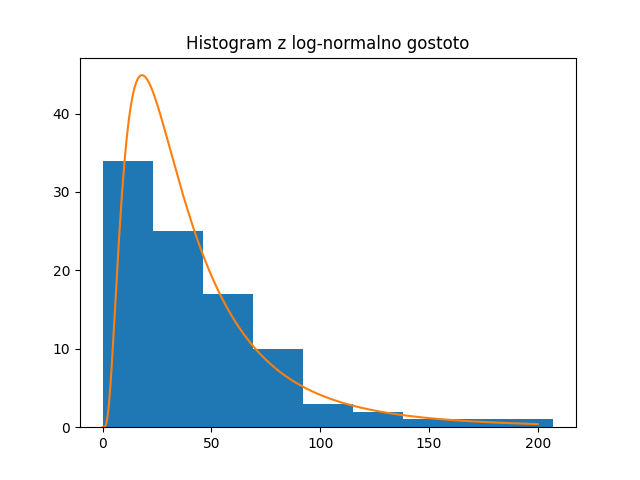
\includegraphics[width=0.7\textwidth]{Histogram1.png}
\end{figure}

Sedaj narišimo še histogram na logaritemski lestvici in dorišimo še ustrezno normalno gostoto. Če uporabimo modificirano Freedman–
Diaconisovo pravilo, da določimo širino razreda desetiških logaritmov, ugotovimo, da morajo biti razredi širine $0.282$. Dobimo naslednji histogram.

\begin{figure}[H]
    \centering
    %\caption{Histogram 2}
    \label{fig:hist1}
    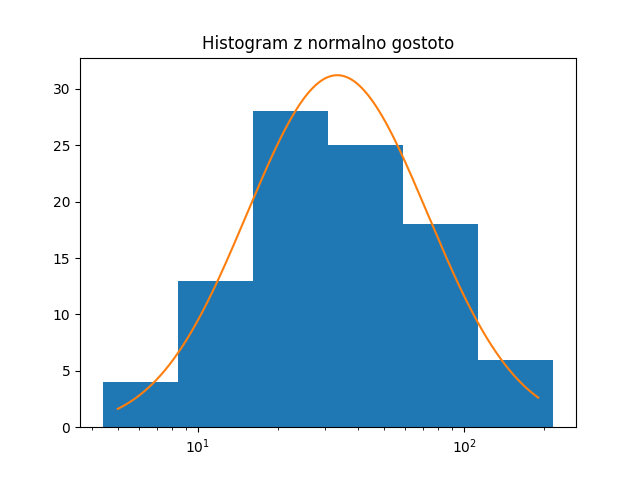
\includegraphics[width=0.7\textwidth]{Histogram2.png}
\end{figure}

Vidimo, da se pri obeh histogramih podatki o hrbtnih dolžinah hobotnic dobro prilegajo ustreznima gostotama.

Nazadnje primerjajmo podatke z log-normalno gostoto še s primerjalnim kvantilnim (Q–Q) grafikonom. Na grafikonu bomo obe osi prikazali na logaritemski lestvici.

\begin{figure}[H]
    \centering
    %\caption{Q-Q grafikon}
    \label{fig:hist1}
    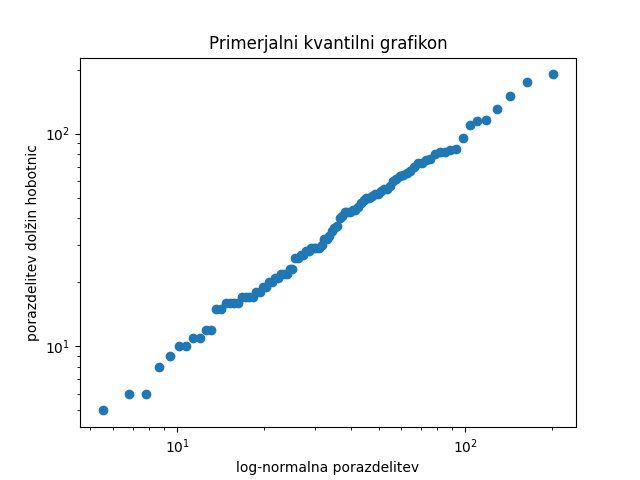
\includegraphics[width=0.7\textwidth]{PrimerjalniGrafikon.png}
\end{figure}

Točke na tem grafikonu ležijo približno na premici. Sklepamo, da so torej podatki res približno v skladu z log-normalnim modelom.

Pri tej nalogi smo uporabljali program \textbf{hobotnice.py}. Ta program zgenerira ob histograma in primerjalni kvantilni grafikon, hkrati pa izpiše naslednji izhod:

\begin{verbatim}
širina po modificiranem Freedman-Diaconisovem pravilu je 23.016005260370942, ...... (TODO)
\end{verbatim}

\section{Piščanci}
Pri tej nalogi bomo ugotovili, kako se spreminja teža piščanca s časom in ali dieta vpliva na pridobivanje teže piščanca.

\begin{enumerate}[a)]
    \item Oceniti moramo, koliko teže piščanec pridobi vsak dan.
\end{enumerate}

\end{document}